\documentclass[10pt]{beamer}
%\documentclass[handout,10pt]{beamer}  % Remove pauses and disable commands like "onslide"
\usetheme[
%%% options passed to the outer theme
%    hidetitle,           % hide the (short) title in the sidebar
     hideauthor,          % hide the (short) author in the sidebar
%    hideinstitute,       % hide the (short) institute in the bottom of the sidebar
%    shownavsym,          % show the navigation symbols
%    width=2cm,           % width of the sidebar (default is 2 cm)
%    hideothersubsections,% hide all subsections but the subsections in the current section
%    hideallsubsections,  % hide all subsections
    left               % right of left position of sidebar (default is right)
%%% options passed to the color theme
%    lightheaderbg,       % use a light header background
]{SJSUsidebar}

\usepackage{environ}
\usepackage{tikz}
\usepackage{listings} % Used for printing source code in papers
\usepackage{pgfplots}\pgfplotsset{compat=newest} % Used to create graphs
\usepackage[utf8]{inputenc}
\usepackage[english]{babel}
\usepackage[T1]{fontenc}
% Or whatever. Note that the encoding and the font should match. If T1
% does not look nice, try deleting the line with the fontenc.
\usepackage{helvet}
\usepackage{makecell} % Used to create thick links in tables
\usepackage{multirow} % Allows merging rows or columns in a table

%%%%%%%%%%%%%%%%%%%%%%%%%%%%%%%%%%%%%%%%%%
%%   Scales tikz images to slide size   %%
%%%%%%%%%%%%%%%%%%%%%%%%%%%%%%%%%%%%%%%%%%
\makeatletter
\newsavebox{\measure@tikzpicture}
\NewEnviron{scaletikzpicturetowidth}[1]{%
  \def\tikz@width{#1}%
  \def\tikzscale{1}\begin{lrbox}{\measure@tikzpicture}%
  \BODY
  \end{lrbox}%
  \pgfmathparse{#1/\wd\measure@tikzpicture}%
  \edef\tikzscale{\pgfmathresult}%
  \BODY
}
\makeatother
%%%%%%%%%%%%%%%%%%%%%%%%%%%%%%%%%%%%%%%%%%



\title[My Presentation Title]% optional, use only with long paper titles
{\textbf{My Presentation Title}}

\subtitle{}  % could also be a conference name

\date{January 2, 2017}

\author[Zayd Hammoudeh] % optional, use only with lots of authors
{
    Zayd Hammoudeh~\\
    \href{mailto:hammoudeh@gmail.com}{{\tt hammoudeh@gmail.com}}
}
% - Give the names in the same order as they appear in the paper.
% - Use the \inst{?} command only if the authors have different
%   affiliation. See the beamer manual for an example

\institute[
%  {\includegraphics[scale=0.2]{SJSU_segl}}\\ %insert a company, department or university logo
    Dept.\ of Computer Science\\
    San Jos\'{e} State University\\
] % optional - is placed in the bottom of the sidebar on every slide
{% is placed on the title page
    Department of Computer Science\\
    San Jos\'{e} State University\\
  
  %there must be an empty line above this line - otherwise some unwanted space is added between the university and the country (I do not know why;( )
}


\begin{document}
% the titlepage
{
\begin{frame}[plain,noframenumbering]{}{} % the plain option removes the sidebar and header from the title page
	\titlepage
\end{frame}}
%%%%%%%%%%%%%%%%



\section{Thesis Goals}
\begin{frame}{Introduction}{My Intro}
  \onslide<1->{
    \textbf{First Thing}: This appears first
    \vfill
  }
  \onslide<2->{
    \textbf{Other Stuff}:
    \vspace{0.4em}
    \begin{itemize}
      \setlength\itemsep{0.8em}
      \item This thing next
      \item Then this citation~\cite{lilJonOk}
    \end{itemize}    
  }
\end{frame}
%%%%%%%%%%%%%%%%

\subsection{Cat}
\begin{frame}{Introduction}{Jig Swap Puzzles}
    \textbf{Cat} -- Cat
    \vfill
    % Delay the table on the slide
    \begin{tabular}{ 
      >{\centering\arraybackslash}m{0.45\textwidth} >{\centering\arraybackslash}m{0.45\textwidth} }
	    \onslide<2->{
	      \fbox{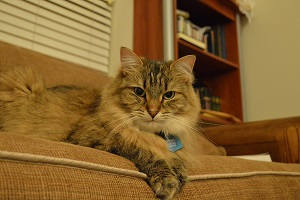
\includegraphics[width=0.365\textwidth]{./images/muffins_300x200.jpg}}
	    } & 
	    \onslide<3->{
	      \fbox{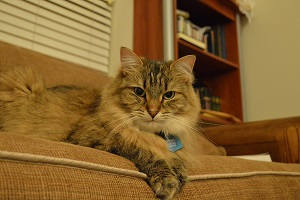
\includegraphics[width=0.365\textwidth]{./images/muffins_300x200.jpg}}
	    }
	    \\ ~\\
	    \onslide<2->{
	      {\small Muffins}
	    } & \onslide<3->{
	      {\small Too Much?}
	    }
	    \\ ~\\
  \end{tabular}
\end{frame}
%%%%%%%%%%%%%%%%


\section{Graph}
\subsection{Graphing in LaTeX}
\begin{frame}{Determining Input Puzzle Count}{Multiple Input Puzzles -- Results}
   \onslide<1->{
     \begin{center}
       \begin{scaletikzpicturetowidth}{0.9\textwidth}
        \begin{tikzpicture}[scale=\tikzscale]
          \begin{axis}[
                ybar, axis on top,
                height=8cm, width=12cm,
            	axis background/.style={fill=gray!10},
                bar width=0.4cm,
                ymajorgrids, tick align=inside,
                major grid style={draw=white},
                enlarge y limits={value=.1,upper},
                ymin=0, ymax=100,
                axis x line*=bottom,
                axis y line*=left,
                y axis line style={opacity=1},
                tickwidth=0pt,
                title=\textbf{Mixed-Bag Solver's Input Puzzle Count Error Frequency},
                enlarge x limits=0.2,
                legend style={
                    at={(0.5,-0.2)},
                    anchor=north,
                    legend columns=-1,
                    /tikz/every even column/.append style={column sep=0.5cm}
                },
                xlabel={Size of Input Puzzle Count Error},
                ylabel={Frequency (\%)},
                symbolic x coords={
                   0, 1, 2, 3},
               xtick=data,
               nodes near coords={
                \pgfmathprintnumber[precision=0]{\pgfplotspointmeta}
               }
            ]
        \addplot [fill=blue!30]
            coordinates {(0,74.5) (1,16.4) (2,7.3) (3,1.8)};
        \addplot [fill=red!30]
            coordinates {(0,44) (1,48) (2,4) (3,4)};
        \addplot [fill=green!30]
            coordinates {(0,50) (1,50) (2,0) (3,0)};
        \addplot [fill=gray]
            coordinates {(0,60) (1,20) (2,20) (3,0)};
        \legend{2 Puzzles, 3 Puzzles, 4 Puzzles, 5 Puzzles}
        \end{axis}
        \end{tikzpicture}
      \end{scaletikzpicturetowidth}  
    \end{center}
  }
\end{frame}
%%%%%%%%%%%%%%%%



%% Optional Table of Contents
\begin{frame}{\textbf{Summary of Topics}}{}
	\tableofcontents
\end{frame}
%%%%%%%%%%%%%%%%



%%%%%%%%%%%%%%%%%%%%%%%%%%%%%%%%%%%%%%%%%%%%%%%%%%%%%%%%%%%%%%%%%%%%
%%%%%%               APPENDIX / BACK-UP SLIDES                %%%%%%
%%%%%%%%%%%%%%%%%%%%%%%%%%%%%%%%%%%%%%%%%%%%%%%%%%%%%%%%%%%%%%%%%%%%

% Stop numbering the slides
\backupbegin

% Add an appendix slide to break up the flow
\appendix

\section*{}  % Close the previous section

\section{Oh No You Didn't}
\subsection{Oh Yes I Did}
\begin{frame}{Word?}{Yep}
  \begin{itemize}
    \setlength\itemsep{.8em}
    \item<1-> I can list stuff
    \begin{itemize}
      \setlength\itemsep{.8em}
    	\item<1-> This shows
    	\item<1-> with this
    \end{itemize}
    \vfill
    \item<2-> Did you forget me?
    \vfill
    \item<3-> How about me?
  \end{itemize}
\end{frame}
%%%%%%%%%%%%%%%%

% Add the list of references
\begin{frame}[t,allowframebreaks]{List of References}
	\bibliographystyle{ieeetr}
	{\tiny \bibliography{references}}
\end{frame}



\backupend



\end{document}
